\section{Measuring Structural Complexity}\label{sec:meaComplex}

THINGS TO DO
\begin{enumerate}
\item rewrite for consistency in notation. For example, some parts of the paper call word length $l$ and some call it $n$.

\item make sure it is clear and we justify that detecting and characterizing structural complexity is hard for real-valued noisy time series.
\item Quantifying structured and unstructured complexity is nontrivial in the case of real-valued noisy time series but WPE does this. [[talk about again here but justify in information theory section]]
\item justify and explain the regime split in \svd 
\end{enumerate}


For the purposes of this paper, one can view entropy as a measure of complexity
and predictability in a time series.  A high-entropy time series is almost
completely unpredictable---and conversely.  This can be made more rigorous:
Pesin's relation \cite{pesin77} states that in chaotic dynamical systems, the
Shannon entropy rate is equal to the sum of the positive Lyapunov exponents,
$\lambda_i$. The Lyapunov exponents directly quantify the rate at which nearby
states of the system will diverge with time: $\left| \Delta x(t) \right| \approx
e^{\lambda t} \left| \Delta x(0) \right|$.  The faster the divergence, the more
difficult prediction becomes.

Utilizing entropy as a measure of temporal complexity is by no means a new idea
\cite{Shannon1951, mantegna1994linguistic}.  Its effective usage requires
categorical data: $x_t \in \mathcal{S}$ for some finite or countably infinite
\emph{alphabet} $\mathcal{S}$, whereas data taken from real-world systems is
effectively real-valued.  To get around this, one must discretize the data---
typically achieved by binning.  Unfortunately, this is rarely a good solution to
the problem, as the binning of the values introduces an additional dynamic on
top of the intrinsic dynamics whose entropy is desired.  The field of symbolic
dynamics studies how to discretize a time series in such a way that the
intrinsic behavior is not perverted, but these methods are fragile in the face
of noise and require further understanding of the underlying system, which
defeats the purpose of measuring the entropy in the first place.

Bandt and Pompe introduced the \emph{permutation entropy} (PE) as a ``natural
complexity measure for time series" \cite{bandt2002per}.  Permutation entropy
employs a method of discretizing real-valued time series that follows the
intrinsic behavior of the system under examination.  Rather than looking at the
statistics of sequences of values, as is done when computing the Shannon
entropy, permutation entropy looks at the statistics of the \emph{orderings} of
sequences of values using ordinal analysis. Ordinal analysis of a time series is
the process of mapping successive time-ordered elements of a time series to
their value-ordered permutation of the same size.  By way of example, if $(x_1,
x_2, x_3) = (9, 1, 7)$ then its \emph{ordinal pattern}, $\phi(x_1, x_2, x_3)$,
is $231$ since $x_2 \leq x_3 \leq x_1$.  This method has many features; among
other things, it is generally robust to observational noise and requires no
knowledge of the underlying mechanisms.

\begin{mydef}[Permutation Entropy]

  Given a time series $\{x_t\}_{t = 1,\dots,T}$. Define $\mathcal{S}_n$ as all
  $n!$ permutations $\pi$ of order $n$. For each $\pi \in \mathcal{S}_n$ we
  determine the relative frequency of that permutation occurring in $\{x_t\}_{t
  = 1,\dots,T}$:
  \begin{align*}
    p(\pi) = \frac{\left|\{t|t \leq T-n,\phi(x_{t+1},\dots,x_{t+n}) = \pi\}\right|}{T-n+1}
  \end{align*}
  Where $|\cdot|$ is set cardinality. The \emph{permutation entropy} of order $n
  \ge 2$ is defined as
  \begin{align*}
  H(n) = - \sum_{\pi \in \mathcal{S}_n} p(\pi) \log_2 p(\pi)
  \end{align*}

\end{mydef}

Notice that $0\le H(n) \le \log_2(n!)$ \cite{bandt2002per}.  With this in mind,
it is common in the literature to normalize permutation entropy as follows:
$\frac{H(n)}{\log_2(n!)}$.  With this convention, ``low'' entropy is close to 0
and ``high'' entropy is close to 1. Finally, it should be noted that the
permutation entropy has been shown to be identical to the Shannon entropy for
many large classes of systems \cite{amigo2012permutation}.

Here we will be utilizing a variation of the permutation entropy, the
\emph{weighted permutation entropy} (WPE)~\cite{fadlallah2013}. The weighted
permutation entropy attempts to correct for observational noise which is larger
than some trends in the data, but smaller than the larger scale features --- for
example, a signal that switches between two fixed points with noise about those
fixed points. The weighted permutation entropy would be dominated by the
switching rather than by the stochastic fluctuation. To accomplish this, the
\emph{weight} of a permutation is taken into account:
\begin{align*}
  w(x_{t+1:t+n}) = \frac{1}{n}
                 \sum_{x_i \in \{x_{t+1:t+n}\}}
                 \left( x_i - \bar{x}_{t+1:t+n} \right)^2
\end{align*}
where $x_{t+1:t+n}$ is a sequence of values $x_{t+1}, \ldots, x_{t+n}$, and
$\bar{x}_{t+1:t+n}$ is the arithmetic mean of those values.

The weighted probability of a permutation is then:
\begin{align*}
  p_w(\pi) = \frac{\displaystyle \sum_{t \le T - n} w(x_{t+1:t+n}) \cdot \delta(\phi(x_{t:t+n}), \pi) }{\displaystyle \sum_{t \le T - n} w(x_{t+1:t+n})}
\end{align*}
where $\delta(x, y)$ is 1 if $x = y$ and 0 otherwise. Effectively, this weighted
probability enhances permutations involved in ``large'' features and demotes
permutations which are small in amplitude relative to the features of the time
series. The weighted permutation entropy is then:
\begin{align*}
  H_w(n) = - \sum_{\pi \in \mathcal{S}_n} p_w(\pi) \log_2 p_w(\pi),
\end{align*}
which can also be normalized by dividing by $\log_2(n!)$, and will be in all the
results of this paper.

In practice, calculating permutation entropy and weighted permutation entropy
involves choosing a good value for the word length $n$. The primary
consideration is that the value be large enough that forbidden ordinals are
discovered, yet small enough that reasonable statistics over the ordinals are
gathered: e.g.:
\begin{align*}
  n = \operatornamewithlimits{argmax}_\ell \{ T \gtrapprox 100 \ell! \},
\end{align*}
assuming an average of 100 counts per ordinal is sufficient. In the literature,
$3 \le n \le 6$ is a standard choice --- generally without any formal
justification. In theory, the permutation entropy should reach an asymptote with
increasing $n$, but that requires an arbitrarily long time series. In practice,
what one should do is calculate the \emph{persistent} permutation entropy by
increasing $n$ until the result converges, but data length issues can intrude
before that convergence is reached.

The weighted permutation entropy for the {\tt SVD} program is given in
Fig.~\ref{fig:wwpe}. To generate this image a window of 5,000 values slid over
the time series. Within each of those windows, the statistics over words of
length 4 are computed and the WPE is calculated. The gray bands denote regions
where the 5,000 value window overlapped visually-distinct regimes. It can be
seen that the behaviors of the weighted permutation entropy vary between
regimes. [[I think here it would be good to add a paragraph explaining the windowed WPE was used for regime choices on SVD...emphasizing  that over a time series permutation entropy fluctuates illustrating within a single time series different levels of complexity and predictability exist. Maybe point at some of the predicting predictability papers.]]

%\begin{figure}[htbp]
%  \centering
%  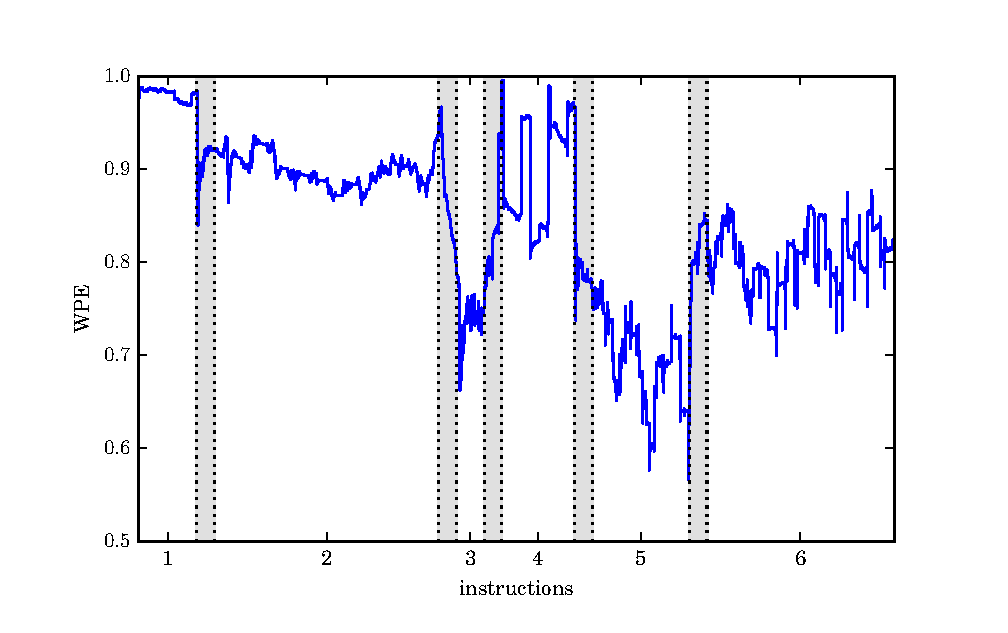
\includegraphics[width=1.0\textwidth]{figs/SVD_wwpe}
%  \caption{[[Joshua: I think adding the colored SVD trace to this would be %good or putting it above this figure]]The weighted permutation entropy of %one run of SVD. The gray bands
%    are regions where the window overlaps regimes. The window size used is
%    $5,000 \times 100,000$ instructions and the word length is $4$.}
%  \label{fig:wwpe}
%\end{figure}


%%FIGURE INTENT
%This figure shows that entropy changs over time with the signal as well as why the regimes for \svd were chosen. 
%%%%%%%%%%%%%%%%%
\begin{figure}[htbp]
  \centering
         
  %\begin{subfigure}{0.3\textwidth}
  %  \includegraphics[width=0.3\textwidth]{figs/svdipcregimescolored.png}
  %  \caption{The instructions per cycle of \svd. Each color corresonds to the different regimes as selected by rapid shifts in WPE, as seen in Figure \ref{fig:svd_wwpe}. From left to right each change in color represents a change in regime for 6 regimes in total. }
 %   \label{fig:svd_ts}
 % \end{subfigure}%
  %\\
 % \begin{subfigure}{\textwidth}
    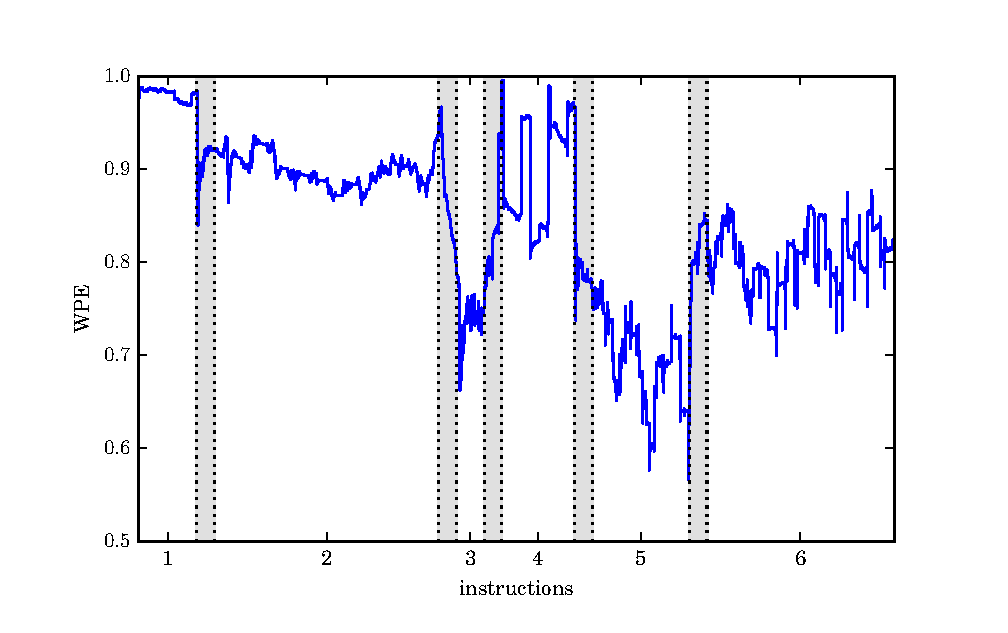
\includegraphics[width=\textwidth]{figs/SVD_wwpe}
    %\caption{The MASE of ARIMA vs weighted permutation entropy. }
  \caption{
[Joshua: I think adding the colored SVD trace to this would be good or putting it above this figure but need to figure how to line them up properly. Also we need to label that the numbers on the bottom of WPE are regimes not instructions...]]The weighted permutation entropy of one run of SVD. The gray bands
    are regions where the window overlaps regimes. The window size used is
    5,000 $\times$ 100,000 instructions and the word length is $4$.[[Joshua:why is $l=4$ and not 5,6 like the rest of the paper?]]For reference the instructions per cycle of \svd are plotted as a ghost behind this plot. Each color on the ghosted time series corresonds to the different regimes as selected by rapid shifts in WPE. From left to right each change in color represents a change in regime for 6 regimes in total.}\label{fig:wwpe}
\end{figure}




